\begin{figure}[htbp]
    \centering
    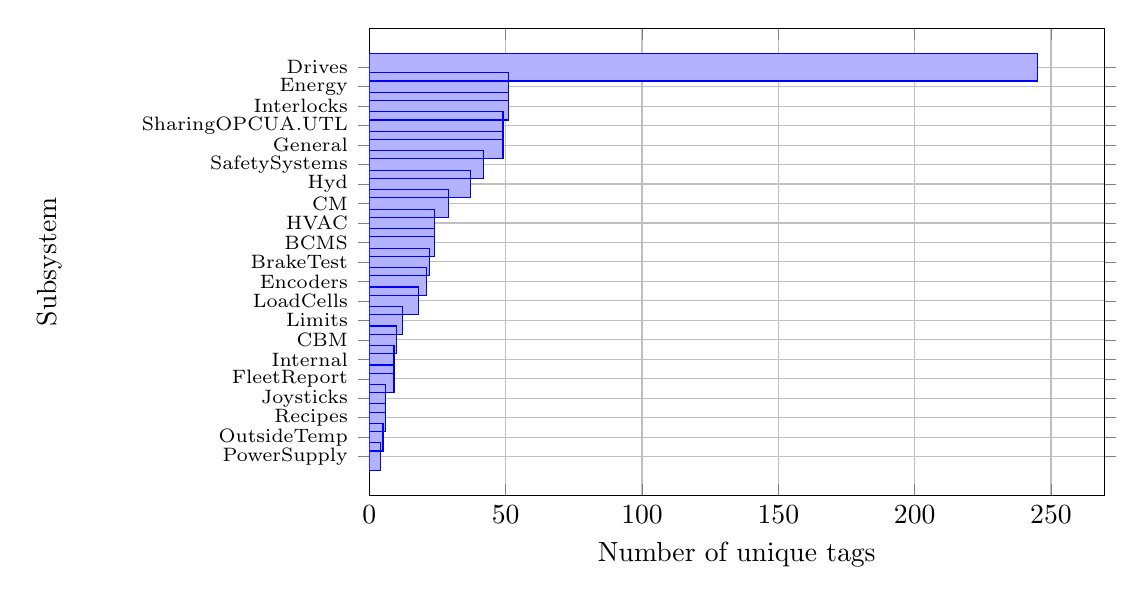
\begin{tikzpicture}
    \begin{axis}[
        width=0.9\linewidth,
        height=0.62\linewidth,
        xbar,
        xlabel={Number of unique tags},
        ylabel={Subsystem},
        y dir=reverse,
        ytick={1,2,3,4,5,6,7,8,9,10,11,12,13,14,15,16,17,18,19,20,21},
        yticklabels={
{Drives},
{Energy},
{Interlocks},
{SharingOPCUA.UTL},
{General},
{SafetySystems},
{Hyd},
{CM},
{HVAC},
{BCMS},
{BrakeTest},
{Encoders},
{LoadCells},
{Limits},
{CBM},
{Internal},
{FleetReport},
{Joysticks},
{Recipes},
{OutsideTemp},
{PowerSupply}
        },
        yticklabel style={font=\scriptsize, text width=0.28\linewidth, align=right},
        xmin=0,
        grid=major
    ]
        \addplot coordinates {
(245,1)
(51,2)
(51,3)
(49,4)
(49,5)
(42,6)
(37,7)
(29,8)
(24,9)
(24,10)
(22,11)
(21,12)
(18,13)
(12,14)
(10,15)
(9,16)
(9,17)
(6,18)
(6,19)
(5,20)
(4,21)
        };
    \end{axis}
    \end{tikzpicture}
    \caption{Number of unique sensor tags by subsystem.}
    \label{fig:subsystem-unique-tags}
\end{figure}
